\section{Generaliseringer af lasso}
\textit{I dette afsnit introduceres nogle generaliseringer af lasso, som alle besidder de to essentielle egenskaber af standard lasso nemlig shrinkage og variable udvægelse.
Afsnittet er skrevet udfra kapitel 4 i \citep{hastie}}

Selvom lasso har vist succes i mange tilfælde, har den også nogle begrænsninger. Dette beskrives i tre scenarier i \citep{zou_hastie} . 
\begin{itemize}
\item Hvis $p>n$, da udvælger lasso højst $n$ variabler eftersom lasso er et konvekst optimeringsproblem. Derudover er lasso ikke veldefineret medmindre $\ell_1$-normen af koefficienterne er mindre end en bestemt værdi. 
\item Hvis der er en gruppe af variabler, som har høj parvis korrelation, så har lasso en tildens til at udvælge kun en variable fra gruppen og er ligeglad med hvilken én den udvælger. 
\item Hvis $n>p$ og der er høj korrelerede variabler, er det empirisk bevidst at prædiktions performance af lasso er outperformede af ridge regression \citep{lasso}. 
\end{itemize}

\subsection{Elastisk net}
Elastisk net, som blev introduceret af \citep{zou_hastie}, gør et kompromis mellem strafleddet af ridge regression og strafleddet af lasso.
Det betyder, at metoden er bedre til korreleret grupper og vælger/fravælger de korreleret prediktorer.
Det elastiske net løser det konvekse optimeringsproblem
\begin{align}
\arg \min_{\beta_0, \beta} \cbr{\frac{1}{2n} \sum_{i=1}^n \del{y_i - \beta_0 - x_{i}^T \beta}^2 + \lambda \sbr{\frac{1}{2} (1- \alpha) \Vert \beta \Vert_2^2 + \alpha \Vert \beta \Vert_1}}, \label{eq:4.2}
\end{align}
hvor $\alpha \in [0,1]$ er en parameter, som kan varieres. 

Hvis $\alpha=1$, da reduceres strafleddet til $\ell_1$-normen svarende til strafleddet for lasso, og hvis $\alpha=0$ reduceres det til den kvadrerede $\ell_2$-norm svarende til strafleddet for ridge regression.

For ethvert $\alpha<1$ og $\lambda>0$, da er det elastiske net problem \eqref{eq:4.2} streng konveks, dvs der eksisterer en entydig løsning uanset korrelations strukturen af $X_j$.

Figur \ref{fig:elastisk_net} viser betingelsesområderne for henholdsvis det elastiske net og standard lasso for tre variable.
Heraf ses at det elastiske net har egenskaberne af $\ell_1$ kuglen og $\ell_2$ kuglen: de skarpe hjørner og kanter opfordrer til variable udvælgelse, mens de kurvede konturer opfordrer stærk korreleret variable at dele koefficienterne.
%
\begin{figure}[H]
\centering
 \scalebox{0.5}{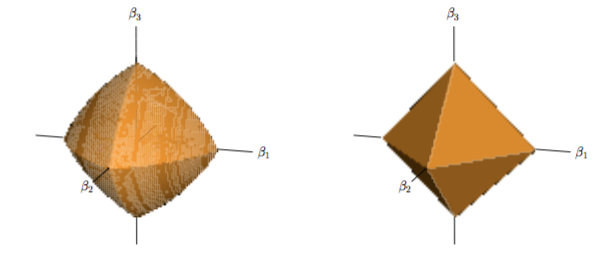
\includegraphics{fig/elastisk_net.jpg}}
\caption{Til venstre ses kuglen for elastisk net med \(\alpha=0.7\) og til højre ses \(\ell_1\) kuglen for \(p=3\).}
\label{fig:elastisk_net}
\end{figure}
%
Det elastiske net har en ekstra tuning parameter $\alpha$, som skal bestemmes.
I praksis kan den ses som en højere-level parameter, og kan sættes udfra en subjektiv vurdering. 
Alternativt, kan man indkludere en sekvens af værdier for $\alpha$ vha krydsvalidering.

Det elastiske net problem \eqref{eq:4.2} er konveks og dermed kan flere optimeringsmetoder anvendes til at løse det.
Coordinate descent er særlig effektiv, og opdateringerne er blot en simpel udvidelse af dem for standard lasso i sektion \ref{sec:lasso_estimatoren}.

Igen centreres prediktorerne \(x_{ij}\), hvoraf den optimale skæring er givet ved \(\hat{\beta}_0=\bar{y}=\frac{1}{n} \sum_{j=1}^n y_j\).
Efter at have løst \(\hat{\beta}_0\), udregnes den optimale vektor \(\hat{\beta}= \del{\hat{\beta}_1, \ldots, \hat{\beta}_p}\).

Coordinate descent opdateringen for $j$'te koefficient er givet ved
\begin{align}
\hat{\beta}_j = \frac{S_{\lambda \alpha} \del{\sum_{i=1}^n r_{ij} x_{ij}}}{\sum_{i=1}^n x_{ij}^2 + \lambda (1-\alpha)}, \label{eq:4.4}
\end{align} 
hvor $S_\mu(z)=\text{sign}(z)(z-\mu)_+$ er soft-thresholding operatoren og $r_{ij}=y_i - \hat{\beta}_0 - \sum_{k \neq j} x_{ik} \hat{\beta}_k$ er den partial residual.
Vi gennemløber opdateringen \eqref{eq:4.4} indtil konvergens.
[Friedman et al (2015)]


\subsection{Grouped lasso}
For mange regressions problemer har kovariaterne en naturlig grupperet struktur, og da foretrækkes det at alle koefficienter indenfor en gruppe er ikke-nul (eller nul) samtidig.
Betragt en lineær regressions model som har $J$ grupper af kovariater, hvor vektoren $Z_j \in \R^{p_j}$ for $j=1, \ldots, J$ repræsenterer kovariaterne i gruppe $j$.
Formålet er da at prædiktere responsvariablen $Y \in \R$ baseret på en samling af kovariater $(Z_1,\ldots,Z_J)$.
En lineær model for regressions funktionen $\E{Y \vert Z}$ er givet ved \(\theta_0 + \sum_{j=1}^J Z_j^T \theta_j\), hvor $\theta_j \in \R^{p_j}$ repræsenterer en gruppe af $p_j$ regressions koefficienter. 

Given en samling af $n$ samples \(\{(y_i, z_{i,1}, z_{i,2}, \ldots, z_{i,J})\}_{i=1}^n\) løser group lasso følgende konveks problem
\begin{align}
\arg \min_{\theta_0 \in \R, \ \theta_j \in \R^{p_j}} \cbr{\frac{1}{2} \sum_{i=1}^n \del{y_i - \theta_0 - \sum_{j=1}^J z_{ij}^T \theta_j}^2 + \lambda \sum_{j=1}^J \Vert \theta_j \Vert_2},\label{eq:4.5}
\end{align}
hvor $\Vert \theta_j \Vert_2$ er den euklidiske norm af vektoren $\theta_j$.
Dette er en grupperet generalisering af lasso, som har følgende egenskaber:
\begin{itemize}
\item Afhængig af $\lambda$, vil enten alle indgange i vektoren $\hat{\theta}_j$ være nul eller ikke-nul
\item Når $p_j=1$, da har vi at $\Vert \theta_j \Vert_2 = \vert \theta_j \vert$, således at alle grupper er singletons, dermed reduceres optimerings problemet \eqref{eq:4.5} til standard lasso problemet.
\end{itemize}
Figur \ref{fig:elastisk_net} viser betingelsesområderne for henholdsvis den grupperet lasso og standard lasso for tre variable.
Vi ser at den grupperet lasso deler egenskaber med både $\ell_1$ og $\ell_2$ kuglen.
%
\begin{figure}[H]
\centering
 \scalebox{0.5}{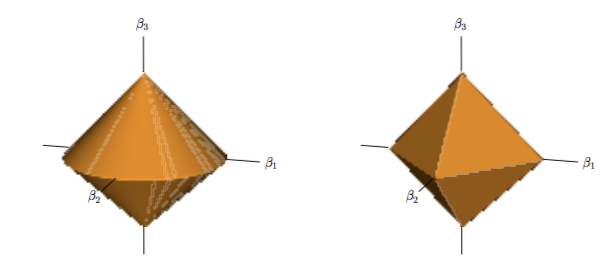
\includegraphics{fig/group_lasso.jpg}}
\caption{Til venstre ses kuglen for elastisk net med \(\alpha=0.7\) og til højre ses \(\ell_1\) kuglen for \(p=3\).}
\label{fig:elastisk_net}
\end{figure}
%
I \eqref{eq:4.5}, straffes alle grupper ligeligt, hvilket betyder at større grupper vil have en tendens til at blive valgt.


\subsubsection{Udregning af group lasso}
Lad os omsrive optimerings problemet \eqref{eq:4.5} på matrix-vektor form
\begin{align*}
\arg \min_{\theta_1, \ldots, \theta_J} \cbr{\frac{1}{2} \Vert \y - \sum_{j=1}^J \mathbf{Z}_{j} \theta_j \Vert_2^2 + \lambda \sum_{j=1}^J \Vert \theta_j \Vert_2}.
\end{align*}
Vi ignorerer skæringen $\theta_0$, da vi centrerer variablerne og responsvariablen.
For dette problem er nul subgradient ligningerne givet ved
\begin{align*}
- \mathbf{Z}_{j}^T \del{\y - \sum_{\ell=1}^J \mathbf{Z}_\ell \hat{\theta}_\ell} + \lambda \hat{s}_j = 0, \quad j=1,\ldots, J,
\end{align*} 
hvor $\hat{s}_j \in \R^{p_j}$ er et element af subdifferentialet af normen $\Vert \cdot \Vert_2$ evalueret i $\hat{\theta}_j$.
Når $\hat{\theta}_j \neq 0$ da har vi, at $\hat{s}_j = \frac{\hat{\theta}_j}{\Vert \hat{\theta}_j \vert_2}$, og når $\hat{\theta}_j=0$ da har vi, at $\hat{s}_j$ er enhver vektor hvor $\Vert \hat{s}_j \Vert_2 \leq 1$.
En metode at løse nul subgradent ligningerne er ved at fastholde alle block vektorer $\{\hat{\theta}_k, k \neq j\}$, og da løse for $\hat{\theta}_j$.
Hermed udføres block coordinate descent på objektfunktionen af group lasso.
Da problemet er konveks, og strafleddet kan separeres efter block, er det garanteret at konvergere til en optimal løsning.
Med $\{\hat{\theta}_k, k \neq j\}$ fastholdt, kan vi skrive
\begin{align*}
- \mathbf{Z}_{j}^T \del{\mathbf{r}_j - \mathbf{Z}_j \hat{\theta}_j} + \lambda \hat{s}_j = 0,
\end{align*}
hvor $\mathbf{r}_j = \y - \sum_{k \neq j} \mathbf{Z}_k \hat{\theta}_k $ er den j'te partial residual.
Fra betingelserne opfyldt af subgradienten $\hat{s}_j$, må vi have at $\hat{\theta}_j =0$ hvis $\Vert \mathbf{Z}_j^T \mathbf{r}_j \Vert_2 < \lambda$, og ellers må $\hat{\theta}_j$ opfylde
\begin{align}
\hat{\theta}_j = \del{\mathbf{Z}_j^T \mathbf{Z}_j + \frac{\lambda}{\Vert \hat{\theta}_j \Vert_2} \mathbf{I}}^{-1} \mathbf{Z}_j^T \mathbf{r}_j. \label{eq:4.14}
\end{align}
Denne opdatering er ens med løsningen af ridge regression, bortset fra at den underliggende straf parameter afhænger af $\Vert \hat{\theta}_j \Vert_2$.
Desværre har ligning \eqref{eq:4.14} ikke en lukket løsning for $\hat{\theta}_j$ medmindre at $\mathbf{Z}_j$ er ortonormal. I dette special tilfælde har vi, at
\begin{align*}
\hat{\theta}_j = \del{1 - \frac{\lambda}{\Vert \mathbf{Z}_j^T \mathbf{r}_j \Vert_2}}_+  \mathbf{Z}_j^T \mathbf{r}_j.
\end{align*}

\subsection{Ikke-konvekse strafled}

tilpasse modeller som er mere sparse end lasso
Den vægtede lasso løser
\begin{align*}
\arg \min_{\beta \in \R^p} \cbr{\frac{1}{2} \Vert \y - \X \beta \Vert_2^2 + \lambda \sum_{j=1}^p w_j \vert \beta_j \vert},
\end{align*}
hvor $w_j = \frac{1}{\vert \tilde{\beta}_j \vert^\nu}$.
Strafleddet for den vægtede lasso kan ses som en approksimation til $\ell_q$ strafleddene med $q=1-\nu$.

\citep{adaptive}
\begin{thm}\label{thm:ALoracle}
Antag $\frac{\lambda_n}{\sqrt{n}} \rightarrow 0$ og $\lambda_n n^\frac{\gamma-1}{2} \rightarrow \infty$. Da må adaptive lasso estimaterne opfylde følgende:
\begin{itemize}
\item Udvælgelsen af variabler er konsistent: $\lim_{n \rightarrow \infty} P(\mathcal{A}_n^\text{AL}=\mathcal{A})=1$
\item Asymptotisk normalitet: $\sqrt{n}\left( \hat{\boldsymbol{\beta}}_\mathcal{A}^{\text{AL}}-\boldsymbol{\beta}_\mathcal{A}^* \right) \overset{d}{\rightarrow} N(\textbf{0},\sigma^2 \boldsymbol{Q}_{11}^{-1}).$
\end{itemize} 
\end{thm}
\begin{proof}
Først bevises asymptotisk normalitet. Lad $\boldsymbol{\beta}=\boldsymbol{\beta}^{*} +\frac{\textbf{u}}{\sqrt{n}}$ og
\begin{align*}
\Psi_n(\textbf{u})=\left\Vert \mathbf{y}-\sum_{j=1}^p \textbf{x}_j \left( \beta_j^{*} +\frac{u_j}{\sqrt{n}} \right) \right\Vert^2 + \lambda_n \sum_{j=1}^p \hat{w}_j \left\vert \beta_j^{*} + \frac{u_j}{\sqrt{n}} \right\vert.
\end{align*}
Lad $\hat{\textbf{u}}^{(n)}=\arg \min \Psi_n(\textbf{u})$, da er $\hat{\boldsymbol{\beta}}^{{\text{AL}}}=\boldsymbol{\beta}^{*} + \frac{\hat{\boldsymbol{u}}^{(n)}}{\sqrt{n}}$ eller $\hat{\boldsymbol{u}}^{(n)}=\sqrt{n}\left(\hat{\boldsymbol{\beta}}^{\text{AL}}-\boldsymbol{\beta}^{*}\right)$.
Lad $V(\mathbf{u})^{(n)}=\Psi_n(\textbf{u}) - \Psi_n(\textbf{0})$, da gælder, at
\begin{align*}
V(\mathbf{u})^{(n)}= \left\Vert \textbf{y} - \sum_{j=1}^p \textbf{x}_j \left( \beta_j^{*} + \frac{u_j}{\sqrt{n}} \right) \right\Vert^2 +
\lambda_n \sum_{j=1}^p \hat{w_j} \left\vert \beta_j^{*} + \frac{u_j}{\sqrt{n}} \right\vert 
-
\left\Vert \textbf{y} - \sum_{j=1}^p \textbf{x}_j \beta_j^{*} \right\Vert^2 - \lambda_n \sum_{j=1}^p \hat{w_j} \left\vert \beta_j^{*} \right\vert. 
\end{align*}
Vi opdeler ligningen og ser først på leddene hvori strafparametrene indgår
\begin{align*}
\lambda_n \sum_{j=1}^p \hat{w_j} \left\vert \beta_j^{*} + \frac{u_j}{\sqrt{n}} \right\vert- \lambda_n \sum_{j=1}^p \hat{w_j} \left\vert \beta_j^{*} \right\vert 
= \lambda_n \sum_{j=1}^p \hat{w_j} \left( \left\vert \beta_j^{*} + \frac{u_j}{\sqrt{n}} \right\vert - \left\vert \beta_j^{*} \right\vert
\right).
\end{align*}
Vi ser herefter på de to resterende led
\begin{align*}
\left\Vert \textbf{y} - \sum_{j=1}^p \textbf{x}_j \left( \beta_j^{*} + \frac{u_j}{\sqrt{n}} \right) \right\Vert^2 -\left\Vert \textbf{y} - \sum_{j=1}^p \textbf{x}_j \beta_j^{*} \right\Vert^2,
\end{align*}
som kan skrives på matrix-vektor form
\begin{align*}
\left(
\textbf{y}-\textbf{X}\boldsymbol{\beta}^{*} -\frac{\textbf{X}\textbf{u}}{\sqrt{n}}
\right)^2 - \left( \textbf{y} - \textbf{X} \boldsymbol{\beta}^{*} \right)^2  & = \left( \textbf{y} - \textbf{X} \boldsymbol{\beta}^{*} \right)^2 + \left( \frac{\mathbf{X}\mathbf{u}}{\sqrt{n}} \right)^2- 2 \left( \textbf{y} - \textbf{X} \boldsymbol{\beta}^{*} \right)^T \left( \frac{\mathbf{X}\mathbf{u}}{\sqrt{n}} \right) - \left( \textbf{y} - \textbf{X} \boldsymbol{\beta}^{*} \right)^2 \\
& = \frac{\textbf{u}^T (\textbf{X}^T\textbf{X})  \textbf{u}}{n} - 2 \boldsymbol{\epsilon}^T \left( \frac{\mathbf{X}\mathbf{u}}{\sqrt{n}} \right) \\ 
&= \textbf{u}^T \left(\frac{1}{n}\textbf{X}^T\textbf{X}\right)  \textbf{u}- 2 \frac{\boldsymbol{\epsilon}^T \textbf{X}}{\sqrt{n}}\textbf{u}.
\end{align*}
Vi får så, at 
\begin{align}
V(\mathbf{u})^{(n)} & = \textbf{u}^T \left(\frac{1}{n}\textbf{X}^T\textbf{X}\right)  \textbf{u} - 2 \frac{\boldsymbol{\epsilon}^T \textbf{X}}{\sqrt{n}}\textbf{u} + \lambda_n \sum_{j=1}^p \hat{w}_j \left( \left\vert \beta_j^{*} + \frac{u_j}{\sqrt{n}} \right\vert - \left\vert \beta_j^{*}\right\vert
\right) \nonumber \\
 & = \textbf{u}^T \left(\frac{1}{n}\textbf{X}^T\textbf{X}\right)  \textbf{u} - 2 \frac{\boldsymbol{\epsilon}^T \textbf{X}}{\sqrt{n}}\textbf{u} +\frac{\lambda_n}{\sqrt{n}} \sum_{j=1}^p \hat{w}_j \sqrt{n} \left( \left\vert \beta_j^{*} + \frac{u_j}{\sqrt{n}} \right\vert - \left\vert \beta_j^{*} \right\vert
\right). \label{eq:V_4}
\end{align}
%
Af antagelse \ref{ant:tvaer}.d) har vi, at der for første led i \eqref{eq:V_4} gælder, at $\frac{1}{n} \mathbf{X}^T \mathbf{X} \overset{p}{\rightarrow} \mathbf{Q}$, mens det for andet led følger af antagelse \ref{ant:tvaer}.f), at $\frac{\boldsymbol{\epsilon}^T \mathbf{X}}{\sqrt{n}} \overset{d}{\rightarrow} \textbf{W}=N(\textbf{0},\sigma^2 \boldsymbol{Q})$. Derfor ser vi nu blot på sidste led i \eqref{eq:V_4}. \\
Hvis $\beta_j^{*} \neq 0$, da har vi, at $\hat{w}_j \overset{p}{\rightarrow} \left\vert \beta_j^{*} \right\vert^{-\gamma}$. Yderligere har vi, at 
\begin{align*}
\lim_{n\rightarrow \infty}
\frac{\left\vert \beta_j^{*} +\frac{u_j}{\sqrt{n}} \right\vert - \left\vert \beta_j^{*} \right\vert}{\frac{u_j}{\sqrt{n}}} =\frac{d}{d \beta_j^{*}} \left\vert \beta_j^{*} \right\vert =\text{sign}\left(\beta_j^{*} \right),
\end{align*} 
hvoraf der gælder, at $\lim_{n\rightarrow \infty} \sqrt{n} \left( \left\vert \beta_j^{*} +\frac{u_j}{\sqrt{n}} \right\vert - \left\vert \beta_j^{*} \right\vert \right) = u_j \text{sign}\left(\beta_j^{*} \right)$.
Af Slutskys sætning \ref{thm:sluktsky} har vi, at 
\begin{align*}
\frac{ \lambda_n}{\sqrt{n}} \hat{w}_j \sqrt{n} \left(\left\vert \beta_j^{*} +\frac{u_j}{\sqrt{n}} \right\vert - \left\vert \beta_j^{*} \right\vert \right) \overset{p}{\rightarrow} 0.
\end{align*}
Hvis $\beta_j^{*} = 0$, da har vi $\sqrt{n} \left( \left\vert \beta_j^{*} +\frac{u_j}{\sqrt{n}} \right\vert - \left\vert \beta_j^{*} \right\vert \right) = \left\vert u_j \right\vert$.
Da $\gamma >0$ kan vægtene omskrives til 
\begin{align*}
\hat{w}_j= \left( \frac{1}{\left\vert \hat{\beta}_j \right\vert} \right)^\gamma=\left( \frac{\sqrt{n}}{\sqrt{n} \left\vert \hat{\beta}_j \right\vert} \right)^\gamma = \frac{n^{\gamma/2}}{ \left( \sqrt{n} \left\vert \hat{\beta}_j \right\vert \right)^\gamma},
\end{align*} 
hvor $\hat{\beta}_j$ er rod-$n$-konsistent. Heraf har vi, at $\frac{\lambda_n}{\sqrt{n}} \hat{w}_j = \frac{\lambda_n}{\sqrt{n}} \frac{n^{\gamma/2}}{\vert \sqrt{n} \hat{\beta}_j \vert^\gamma} = \lambda_n n^{\frac{\gamma -1}{2}} \frac{1}{\vert \sqrt{n} \hat{\beta}_j \vert^\gamma} $, hvor $\sqrt{n} \hat{\beta}_j = O_p(1)$ og vi ved at  $\lambda_n n^\frac{\gamma-1}{2} \rightarrow \infty$, da har vi, at $\frac{\lambda_n}{\sqrt{n}} \hat{w}_j  \vert u_j \vert \rightarrow \infty$.
Af Slutsky sætning ser vi, at $V^{(n)} (\mathbf{u}) \overset{d}{\rightarrow} V(\textbf{u})$ for alle $\mathbf{u}$, hvor
\begin{align*}
V(\textbf{u}) = \begin{cases}
    \mathbf{u}_\mathcal{A}^T \mathbf{Q}_{11} \mathbf{u}_\mathcal{A}-2\mathbf{u}^T_\mathcal{A} \mathbf{W}_\mathcal{A} & \text{hvis  $u_j=0, \ \forall j \notin \mathcal{A} $},\\
    \infty & \text{hvis } \exists u_j \neq 0, \ j \notin \mathcal{A} .
  \end{cases}
\end{align*}
Da funktionen $V^{(n)}$ er konveks, og $(\mathbf{Q}_{11}^{-1} \mathbf{W_\mathcal{A}},0)^T$ er et entydig minimum af $V$, følger det af \cite{Zou} at 
$\arg\min V^{(n)} \rightarrow \arg\min V$.
Derfor får vi
\begin{align}
\hat{\mathbf{u}}_\mathcal{A}^{(n)} \overset{d}{\rightarrow} \mathbf{Q}_{11}^{-1} \mathbf{W}_\mathcal{A} \quad \text{og} \quad \hat{\mathbf{u}}_{\mathcal{A}^C}^{(n)} \overset{d}{\rightarrow} \mathbf{0}. \label{eq:minUA}
\end{align}
Vi observerer, at $\mathbf{W}_\mathcal{A}=N(\mathbf{0}, \sigma^2 \mathbf{Q}_{11})$. \\

Herefter vil vi bevise at udvælgelsen af variabler er konsistent. For alle $j \in \mathcal{A}$, giver den asymptotiske normalitet at $\hat{\beta}_j^{\text{AL}} \overset{p}{\rightarrow}\beta_j^{*}$, dvs. $P(j \in \mathcal{A}_n^{\text{AL}}) \rightarrow 1$. Derfor vil vi vise at $\forall j' \notin \mathcal{A}$, da vil $P(j' \in \mathcal{A}_n^{\text{AL}}) \rightarrow 0$. \\
Vi betragter $j' \in \mathcal{A}_n^{\text{AL}}$ således at $\hat{\beta}_{j'}^{\text{AL}} \neq 0$. Af første ordens betingelser har vi, at 
\begin{align*}
2 \mathbf{x}_{j'}^T  \left( \mathbf{y}-\mathbf{X}\hat{\boldsymbol{\beta}}^{\text{AL}} \right)=\lambda_n \hat{w}_{j'} \left\vert \text{sign}(\hat{\beta}_{j'}^\text{AL}) \right\vert,
\end{align*}
som er ækvivalent med
\begin{align*}
2 \frac{\mathbf{x}_{j'}^T \left( \mathbf{y}-\mathbf{X}\hat{\boldsymbol{\beta}}^{{\text{AL}}}\right)}{\sqrt{n}}=\frac{\lambda_n}{\sqrt{n}} \hat{w}_{j'}.
\end{align*}
Vi fandt, at $\frac{\lambda_n}{\sqrt{n}} \hat{w}_{j'} \overset{p}{\rightarrow} \infty$. Vi har da, at 
\begin{align*}
2 \frac{\mathbf{x}_{j'}^T \left(\mathbf{y}-\mathbf{X}\hat{\boldsymbol{\beta}}^{{\text{AL}}} \right)}{\sqrt{n}}
 &= 2 \frac{\mathbf{x}_{j'}^T \left(\mathbf{X}\boldsymbol{\beta}^*+\boldsymbol{\epsilon}-\mathbf{X}\hat{\boldsymbol{\beta}}^{{\text{AL}}} \right) }{\sqrt{n}} \\
&= 2 \frac{\mathbf{x}_{j'}^T \mathbf{X} \left(\boldsymbol{\beta}^*-\hat{\boldsymbol{\beta}}^{\text{AL}} \right)}{\sqrt{n}}+2\frac{\mathbf{x}_{j'}^T \boldsymbol{\epsilon}}{\sqrt{n}} \\
&= 2 \frac{\mathbf{x}_{j'}^T \mathbf{X} \sqrt{n} \left(\boldsymbol{\beta}^*-\hat{\boldsymbol{\beta}}^{\text{AL}}\right)}{n}+2\frac{\mathbf{x}_{j'}^T \boldsymbol{\epsilon}}{\sqrt{n}}.
\end{align*}
Af \eqref{eq:minUA} og Slutskys sætning \ref{thm:sluktsky}, ved vi at $ 2 \frac{\mathbf{x}_{j'}^T \mathbf{X} \sqrt{n} \left(\boldsymbol{\beta}^*-\hat{\boldsymbol{\beta}}^{\text{AL}}\right)}{n}$ konvergerer i fordeling mod en normalfordeling og $2\frac{\mathbf{x}_{j'}^T \boldsymbol{\epsilon}}{\sqrt{n}} \overset{d}{\rightarrow} N \left(\mathbf{0}, 4 \Vert \mathbf{x}_{j'} \Vert^2 \sigma^2 \right)$. Dvs.
\begin{align*}
P\left(j' \in \mathcal{A}_n^{\text{AL}}\right) \leq P\left(2 \mathbf{x}_{j'}^T \left(\mathbf{y}-\mathbf{X} \hat{\boldsymbol{\beta}}^{\text{AL}}\right)=\lambda_n \hat{w}_{j'} \right) \rightarrow 0.
\end{align*}
\end{proof}


Adaptive elastic net
